\chapter{Tutorial: Processing Mars Orbiter Camera Imagery}
\label{ch:moc_tutorial}

\definecolor{lgray}{gray}{0.95}

\section{Quick Start}
\label{quickstart}

The Stereo Pipeline package contains GUI and command-line programs that
convert a stereo pair in the ISIS {\em cube} format into a 3D ``point
cloud'' image.  This is an intermediate format that can be passed along
to one of several programs that convert a point cloud into a mesh for 3D
viewing, a gridded digital elevation model (DEM) for GIS purposes, or a
LAS/LAZ point cloud.

There are a number of ways to fine-tune parameters and analyze the
results, but ultimately this software suite takes images and builds
models in a mostly automatic way.  To create a point cloud file, you
simply pass two image files to the \texttt{stereo} command:

\begin{verbatim}
  ISIS 3> stereo left_input_image.cub right_input_image.cub stereo-output
\end{verbatim}

Alternatively, the \texttt{stereo\_gui} frontend can be invoked, with
the same options, as described in section \ref{stereo_gui}. This tool
makes it possible to select small clips on which to run \texttt{stereo}.

The string \texttt{stereo-output} is an arbitrary output prefix, it is
used when generating names for \texttt{stereo} output files. For
example, it can be set to \texttt{results/output}, in which case all
output files will be in the \texttt{results} directory and start with
the prefix \texttt{output}. See section \ref{running-stereo} for a more
detailed discussion.

You can then make a visualizable mesh or a \ac{DEM} file with the following
commands (the \texttt{\textit{stereo-output}-PC.tif} and
\texttt{\textit{stereo-output}-L.tif} files are created by the
\texttt{stereo} program above):

\begin{verbatim}
  ISIS 3> point2mesh stereo-output-PC.tif stereo-output-L.tif
  ISIS 3> point2dem  stereo-output-PC.tif
\end{verbatim}

More details are provided in section \ref{visualising}.

\section{Preparing the Data}

The data set that is used in the tutorial and examples below is a
pair of Mars Orbital Camera (\ac{MOC}) \citep{1992JGR....97.7699M,2001JGR...10623429M}
images whose \ac{PDS} Product IDs are M01/00115 and E02/01461.
This data can be downloaded from the PDS directly, or they can be
found in the \texttt{examples/MOC} directory of your Stereo Pipeline distribution.

\subsection{Loading and Calibrating Images using ISIS}

These raw \ac{PDS} images (\texttt{M0100115.imq} and \texttt{E0201461.imq})
need to be imported into the \ac{ISIS} environment and radiometrically
calibrated.  You will need to be in an \ac{ISIS} environment (have
set the \texttt{ISISROOT} environment variable and sourced the
appropriate \ac{ISIS} 3 startup script, as detailed in the \ac{ISIS}
3 instructions; we will denote this state with the `\texttt{ISIS
3>}' prompt).  Then you can use the \texttt{mocproc} program, as follows:

\begin{verbatim}
  ISIS 3> mocproc from=M0100115.imq to=M0100115.cub Mapping=NO
  ISIS 3> mocproc from=E0201461.imq to=E0201461.cub Mapping=NO
\end{verbatim}

There are also \texttt{Ingestion} and \texttt{Calibration} parameters
whose defaults are `\texttt{YES}' which will bring the image into the
\ac{ISIS} format and perform radiometric calibration.  By setting the
\texttt{Mapping} parameter to `\texttt{NO}', the resultant file will be
an \ac{ISIS} cube file that is calibrated, but not map-projected.
Note that while we have not explicitly run \texttt{spiceinit}, the
Ingestion portion of \texttt{mocproc} quietly ran \texttt{spiceinit}
for you (you'll find the record of it in the \ac{ISIS} Session Log,
usually written out to a file named \texttt{print.prt}).  Refer to
Figure~\ref{p19-images} to see the results at this stage of
processing.

\begin{figure}[t!]
\begin{minipage}{5.2in}
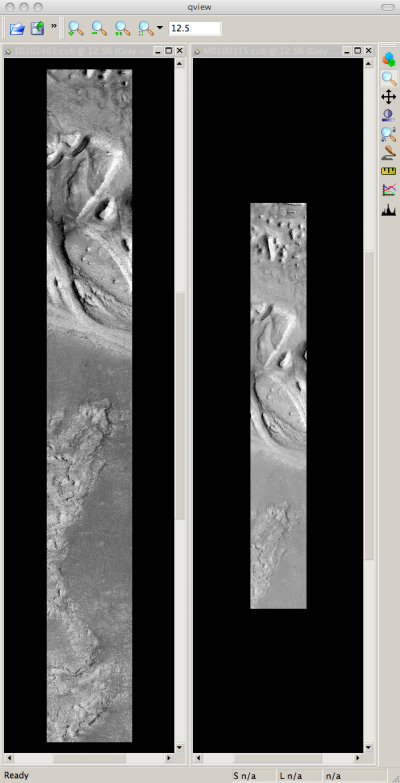
\includegraphics[height=3.7in]{images/p19-images_400px.png}
\hfill
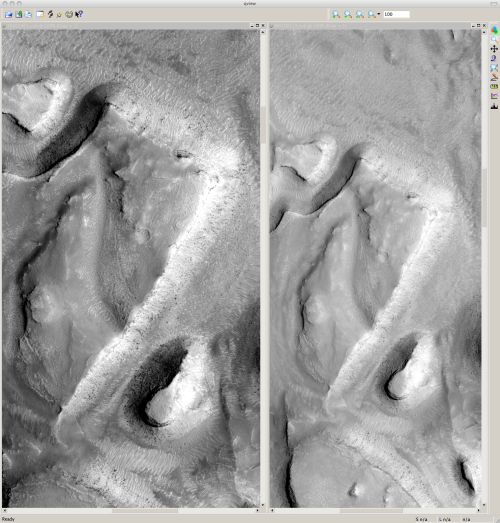
\includegraphics[height=3.7in]{images/p19-images_zoom_500px.png}
\end{minipage}
\hfill
\begin{minipage}{1.3in}
\caption[P19 images open in qview zoomed in]{
    \label{p19-images}
    This figure shows \texttt{E0201461.cub} and \texttt{M0100115.cub}
    open in ISIS's qview program.  The view on the left shows their
    full extents at the same zoom level, showing how they have
    different ground scales.  The view on the right shows both images
    zoomed in on the same feature.  }
\end{minipage}
\end{figure}

Datasets for other type of cameras or other planets can be pre-processed
similarly, using the ISIS tools specific to them.

\subsection{Aligning Images}
\label{sec:AligningImages}

Once the .cub files are obtained, it is possible to run stereo right away,
as
\begin{verbatim}
  ISIS 3> stereo E0201461.cub M0100115.cub    \
            --alignment-method affineepipolar \
            -s stereo.default.example results/output
\end{verbatim}

In this case, the first thing \texttt{stereo} does is to internally
align (or rectify the images), which helps with finding stereo matches.
Here we have used \texttt{affineepipolar} alignment.  Another option is
to use \texttt{homography} alignment, as described in section
\ref{settingoptionsinstereodefault}.

Alternatively, the images can be aligned externally, by map-projecting
them in \ac{ISIS}. External alignment can sometimes give better results
than the simple internal alignment described earlier, especially if the
images are taken from very different perspectives, or if the curvature
of the planet/body being imaged is non-negligible.


We will now describe how to do this alignment, but we also provide the
\texttt{cam2map4stereo.py} program (page \pageref{cam2map4stereo}) which
performs this work automatically for you. (Also note that ASP has its
own internal way of map-projecting images, which we believe is preferable.
That approach is described in section \ref{mapproj-example}.)

The \ac{ISIS} \texttt{cam2map} program will map-project these images:

\begin{verbatim}
  ISIS 3> cam2map from=M0100115.cub to=M0100115.map.cub
  ISIS 3> cam2map from=E0201461.cub to=E0201461.map.cub map=M0100115.map.cub matchmap=true
\end{verbatim}

Notice the order in which the images were run through
\texttt{cam2map}. The first projection with \texttt{M0100115.cub}
produced a map-projected image centered on the center of that image.
The projection of \texttt{E0201461.cub} used the \texttt{map=}
parameter to indicate that \texttt{cam2map} should use the same map
projection parameters as those of \texttt{M0100115.map.cub} (including
center of projection, map extents, map scale, etc.) in creating the
projected image. By map-projecting the image with the worse resolution
first, and then matching to that, we ensure two things: (1) that the
second image is summed or scaled down instead of being magnified up,
and (2) that we are minimizing the file sizes to make processing in
the Stereo Pipeline more efficient.

Technically, the same end result could be achieved by using the
\texttt{mocproc} program alone, and using its \texttt{map=
M0100115.map.cub} option for the run of \texttt{mocproc} on
\texttt{E0201461.cub} (it behaves identically to \texttt{cam2map}).
However, this would not allow for determining which of the two
images had the worse resolution and extracting their minimum
intersecting bounding box (see below).  Furthermore, if you choose
to conduct bundle adjustment (see Chapter \ref{ch:bundle_adjustment},
page \pageref{ch:bundle_adjustment}) as a pre-processing step, you
would do so between \texttt{mocproc} (as run above) and \texttt{cam2map}.

The above procedure is in the case of two images which cover similar
real estate on the ground.  If you have a pair of images where one
image has a footprint on the ground that is much larger than the
other, only the area that is common to both (the intersection of their
areas) should be kept to perform correlation (since non-overlapping
regions don't contribute to the stereo solution).  If the image with
the larger footprint size also happens to be the image with the better
resolution (i.e. the image run through \texttt{cam2map} second with
the \texttt{map=} parameter), then the above \texttt{cam2map}
procedure with \texttt{matchmap=true} will take care of it just fine.
Otherwise you'll need to figure out the latitude and longitude
boundaries of the intersection boundary (with the \ac{ISIS}
\texttt{camrange} program).  Then use that smaller boundary as the
arguments to the \texttt{MINLAT}, \texttt{MAXLAT}, \texttt{MINLON},
and \texttt{MAXLON} parameters of the first run of \texttt{cam2map}.
So in the above example, after \texttt{mocproc} with \texttt{Mapping=
  NO} you'd do this:

\begin{verbatim}
  ISIS 3> camrange from=M0100115.cub
           ... lots of camrange output omitted ...
  Group = UniversalGroundRange
    LatitudeType       = Planetocentric
    LongitudeDirection = PositiveEast
    LongitudeDomain    = 360
    MinimumLatitude    = 34.079818835324
    MaximumLatitude    = 34.436797628116
    MinimumLongitude   = 141.50666207418
    MaximumLongitude   = 141.62534719278
  End_Group
           ... more output of camrange omitted ...
\end{verbatim}

\begin{verbatim}
  ISIS 3> camrange from=E0201461.cub
           ... lots of camrange output omitted ...
  Group = UniversalGroundRange
    LatitudeType       = Planetocentric
    LongitudeDirection = PositiveEast
    LongitudeDomain    = 360
    MinimumLatitude    = 34.103893080982
    MaximumLatitude    = 34.547719435156
    MinimumLongitude   = 141.48853937384
    MaximumLongitude   = 141.62919740048
  End_Group
           ... more output of camrange omitted ...
\end{verbatim}

Now compare the boundaries of the two above and determine the intersection to use as the boundaries for \texttt{cam2map}:

\begin{verbatim}
  ISIS 3> cam2map from=M0100115.cub to=M0100115.map.cub DEFAULTRANGE=CAMERA \
                  MINLAT=34.10 MAXLAT=34.44 MINLON=141.50 MAXLON=141.63
  ISIS 3> cam2map from=E0201461.cub to=E0201461.map.cub map=M0100115.map.cub matchmap=true
\end{verbatim}

You only have to do the boundaries explicitly for the first run of
\texttt{cam2map}, because the second one uses the \texttt{map=}
parameter to mimic the map-projection of the first.  These two
images are not radically different in spatial coverage, so this is not
really necessary for these images, it is just an example.

Again, unless you are doing something complicated, using the
\texttt{cam2map4stereo.py} program (page \pageref{cam2map4stereo})
will take care of all these steps for you.

At this stage we can run the stereo program with map-projected images:

\begin{verbatim}
  ISIS 3> stereo E0201461.map.cub M0100115.map.cub --alignment-method none \
            -s stereo.default.example results/output
\end{verbatim}

Here we have used \texttt{alignment-method none} since
\texttt{cam2map4stereo.py} brought the two images into the same
perspective and using the same resolution. If you invoke
\texttt{cam2map} independently on the two images, without
\texttt{matchmap=true}, their resolutions may differ, and using an
alignment method rather than \texttt{none} to correct for that is still
necessary.

Now you may skip to chapter \ref{nextsteps} which will discuss the
\texttt{stereo} program in more detail and the other tools in ASP.

\chapter{Tutorial: Processing Earth Digital Globe Imagery}
\label{ch:dg_tutorial}

In this chapter we will focus on how to process Earth imagery, or more
specifically Digital Globe data. This is different from our previous
chapter in that at no point will we be using ISIS utilities. This is
because ISIS only supports NASA instruments, while most Earth imagery
comes from commercial providers.

In addition to Digital Globe's satellites, ASP supports any Earth imagery
that uses the RPC camera model format. How to process such data is
described in section \ref{rpc}, although following this tutorial may
still be insightful even if your data is not from Digital Globe.

Digital Globe provides imagery from Quick Bird and the three World
View satellites. These are the hardest images to process with Ames
Stereo Pipeline because they are exceedingly large, much larger than
HiRISE imagery (the GUI interface can be used to run stereo on just a
portion of the images). There is also a wide range of terrain challenges and
atmospheric effects that can confuse ASP. Trees are particularly
difficult for us since their texture is nearly nadir and perpendicular
to our line of sight. It is important to know that the driving force
behind our support for Digital Globe imagery is to create models of
ice and bare rock. That is the type of imagery that we have tested
with and have focused on. If we can make models of wooded or urban
areas, that is a bonus, but we can't provide any advice for how to
perform or improve the results if you choose to use ASP in that way.

ASP can only process Level 1B satellite imagery, and cannot process
Digital Globe's aerial images.

The camera information for Digital Globe images is contained in an XML
file for each image. In addition to the exact linear camera model, the
XML file also has its RPC approximation. In this chapter we will focus
only on processing data using the linear camera model.  For more detail
on RPC camera models we refer as before to section \ref{rpc}.

Our implementation of the linear camera model only models the geometry
of the imaging hardware itself and velocity aberration. We do not
currently model refraction due to light bending in Earth's
atmosphere. It is our understanding that this could represent
misplacement of points up to a meter for some imagery. However this is
still smaller error than the error from measurement of the spacecraft's
position and orientation. The latter can be corrected using bundle
adjustment, ideally used with ground control points (section
\ref{bundleadjust}). Alternatively, the \texttt{pc\_align} tool
discussed in section \ref{pc-align-example} can be used to align the
terrain obtained from ASP to an accurate set of ground
measurements.

In the next two sections we will show how to process unmodified and
map-projected variants of World View imagery. The imagery we are using is
from the free stereo pair example of Guangzhou, China available from
Digital Globe's website \cite{digital-globe:samples}. These images
represent a non-ideal problem for us since this is an urban location,
but at least you should be able to download this imagery yourself and
follow along.

\section{Processing Raw}
\label{rawdg}

After you have downloaded the example stereo imagery of China, you
will find a directory titled

\begin{verbatim}
  053950035030_01_P001_PAN
\end{verbatim}

It has a lot of files and many of them contain redundant information
just displayed in different formats. We are interested only in the TIF
or NTF imagery and the similarly named XML files.

Some Worldview folders will contain multiple image files. 
This is because Digital Globe breaks down a
single observation into multiple files for what we assume are size
reasons. These files have a pattern string of ``\_R[N]C1-'', where N
increments for every subframe of the full observation. The tool named
\texttt{dg\_mosaic} can be used to mosaic (and optionally reduce the
resolution of) such a set of sub-observations into a single image file
and create an appropriate camera file

\begin{verbatim}
    > dg_mosaic 12FEB12053305*TIF --output-prefix 12FEB12053305 --reduce-percent 50
\end{verbatim}

and analogously for the second set. See section \ref{dgmosaic} for more
details. The \texttt{stereo} program can use either the original or the 
mosaicked images.  This sample data only contains two image files so we 
do not need to use the \texttt{dg\_mosaic} tool.

Since we are ingesting these images raw, it is strongly recommended that
you use affine epipolar alignment to reduce the search range. The
\texttt{stereo} command and a rendering of the results are shown below.

\begin{verbatim}
    > stereo -t dg --subpixel-mode 1 --alignment-method affineepipolar \
             13DEC28032941-P1BS-053950035030_01_P001.TIF          \
             13DEC28033039-P1BS-053950035030_01_P001.TIF          \
             13DEC28032941-P1BS-053950035030_01_P001.XML          \
             13DEC28033039-P1BS-053950035030_01_P001.XML dg/dg
\end{verbatim}

Alternatively, the \texttt{stereo\_gui} frontend can be invoked, with
the same options, as described in section \ref{stereo_gui}.

\begin{figure}[h!]
\centering
  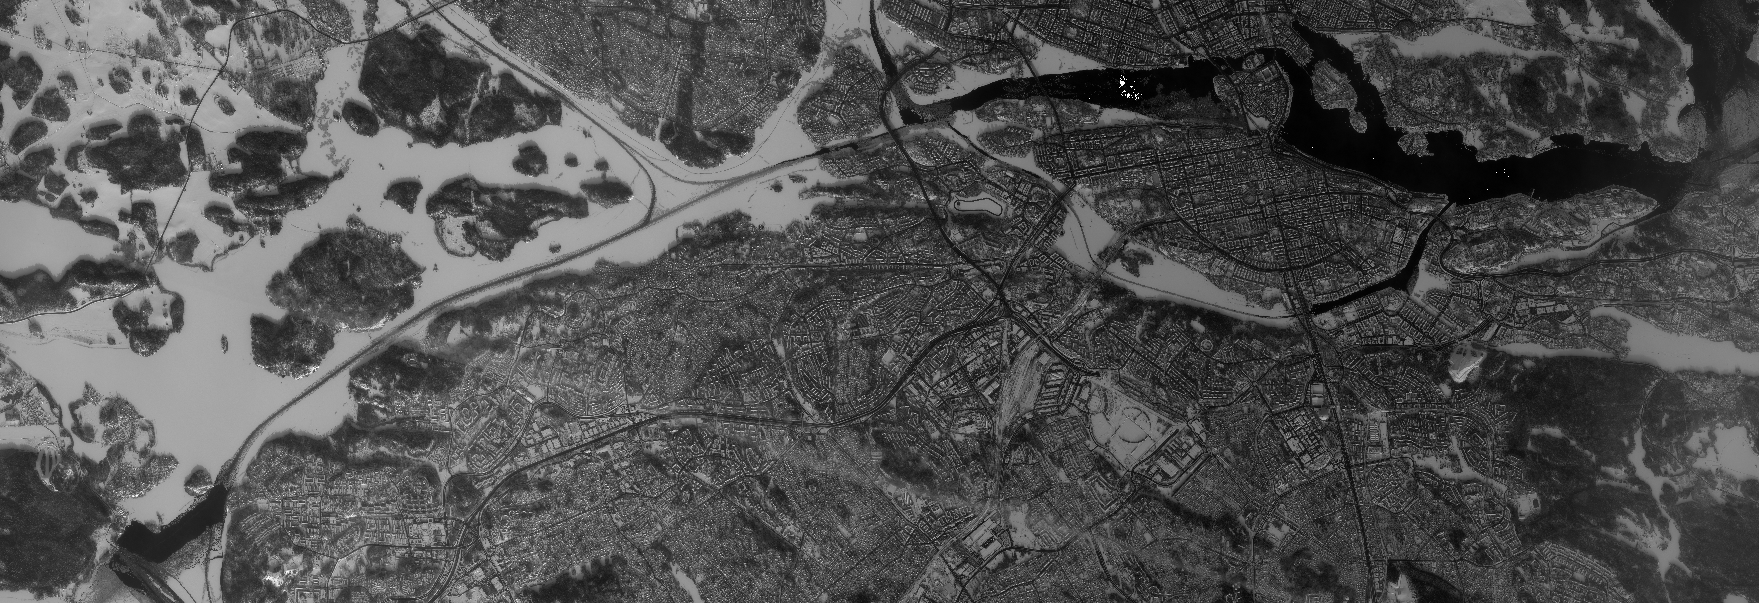
\includegraphics[width=3.0in]{images/examples/dg/wv_tutorial_input.png}
  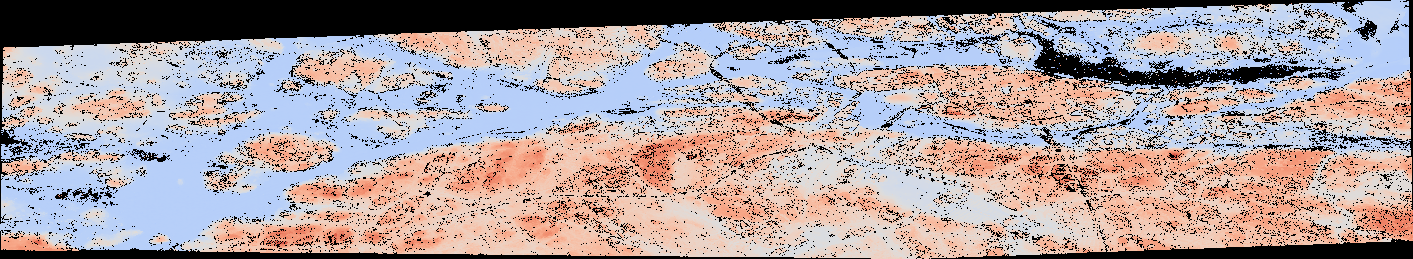
\includegraphics[width=3.0in]{images/examples/dg/wv_tutorial_colormap.png}
\caption{Example WorldView image section and colorized height map.}
\label{fig:dg-nomap-example}
\end{figure}

Above, we have used \texttt{subpixel-mode 1} which is less accurate but
reasonably fast.  More details about how to set this and other
\texttt{stereo} parameters can be found in section
\ref{settingoptionsinstereodefault}.

It is important to note that we could have performed stereo using the
approximate RPC model instead of the exact linear camera model (both
models are in the same XML file), by switching the session in the
\texttt{stereo} command above from \texttt{-t dg} to \texttt{-t
rpc}. The RPC model is somewhat less accurate, so the results will not
be the same, in our experiments we've seen differences in the 3D
terrains using the two approaches of 5 meters or more.

\section{Processing Map-Projected Imagery}
\label{mapproj}

ASP computes the highest quality 3D terrain if used with images map-projected
onto a low-resolution DEM that is used as an initial guess. This process
is described in section \ref{mapproj-example}.

\section{Handling CCD Boundary Artifacts}
\label{wvcorrect-example}

Digital Globe World View images \cite{digital-globe:camera} may exhibit
slight subpixel artifacts which manifest themselves as discontinuities
in the 3D terrain obtained using ASP. We provide a tool named
\texttt{wv\_correct}, that can largely correct such artifacts for World
View-1 and World View-2 images for most TDI. It can be invoked as
follows:

\begin{verbatim}
    > wv_correct image_in.ntf image.xml image_out.tif
\end{verbatim}

The corrected images can be used just as the originals, and the camera
models do not change. When working with such imagery, we recommend that
CCD artifact correction happen first, on original un-projected
imagery. Afterward images can be mosaicked with \texttt{dg\_mosaic},
map-projected, and the resulting data used to run stereo and create
terrain models.

This tool is described in section \ref{wvcorrect}, and an example of
using it is in Figure \ref{fig:ccd-artifact-example}.

\begin{figure}[h!]
\centering
  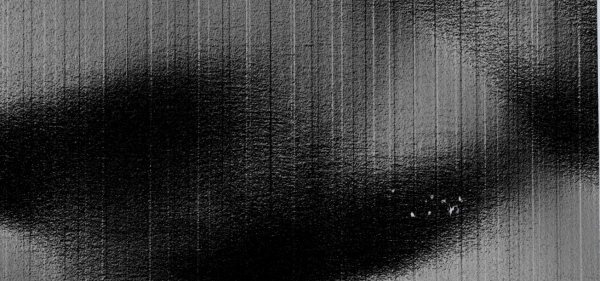
\includegraphics[width=3.0in]{images/examples/ccd_before_600px.png}
  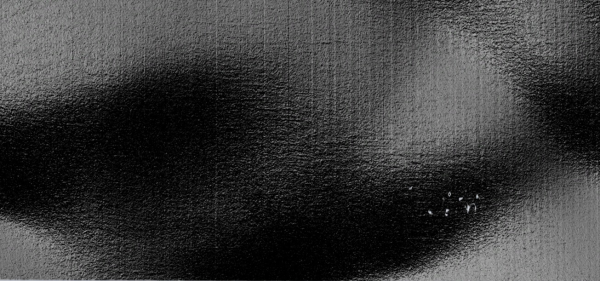
\includegraphics[width=3.0in]{images/examples/ccd_after_600px.png}
\caption{Example of a hill-shaded terrain obtained using stereo without (left) and with (right) CCD boundary artifact corrections applied using \texttt{wv\_correct}.}
\label{fig:ccd-artifact-example}
\end{figure}

\section{Managing Camera Jitter}
\label{sec:jitter}

In this section we will talk about the second largest source of
inaccuracies in Digital Globe imagery, after CCD artifacts, namely
jitter, and how to correct it. 

It is important to note that jitter correction is highly experimental,
and while it usually works, it may not be production-ready. 

The order in which these corrections need to be handled is the following. First,
CCD artifacts are corrected. Then, optionally, images are mosaicked with
\texttt{dg\_mosaic} and map-projected. And jitter should be handled
last, during stereo. An exception is made for WV03 images, for which CCD
artifacts do not appear to have a significant effect.

Camera jitter has its origin in the fact that the measured position and
orientation of the image-acquiring line sensor as specified in a camera
XML file is usually not perfectly accurate, the sensor in fact wiggles
slightly from where it is assumed to be as it travels through space and
appends rows of pixels to the image. This results in slight errors in
the final DEM created using stereo. Those are most clearly seen in the
intersection error map output by invoking \texttt{point2dem -\/-errorimage}.

ASP provides support for correcting this jitter, at least its
lower-frequency component. During stereo, right before the triangulation
step, so after the left-to-right image disparity is computed, it can
solve for adjustments to apply to the satellite position and
orientation. Those adjustments are placed along-track (hence at several
lines in the image) with interpolation between them. This is quite
analogous to what \texttt{bundle\_adjust} is doing, except that the
latter uses just one adjustment for each image.

This process can be triggered by invoking \texttt{stereo} with
\texttt{-\/-image-lines-per-piecewise-adjustment arg}. A recommended
value here is 1000, though it is suggested to try several values. A
smaller value of \texttt{arg} will result in more adjustments being used
(each adjustment being responsible for fewer image lines), hence
providing finer-grained control, though making this number too small may
result in over-fitting and instability. A smaller value here will also
require overall more interest point matches (as computed from the
disparity), which is set via
\texttt{-\/-num-matches-for-piecewise-adjustment}.

Jitter correction is more effective if \texttt{stereo} is preceded by
bundle adjustment, with the adjusted cameras then being passed to \texttt{stereo}
via \texttt{-\/-bundle-adjust-prefix}.

If it appears that the adjustments show some instability at the starting
and ending lines due to not enough matches being present (as deduced
from examining the intersection error image), the locations of the first
and last adjustment (and everything in between) may be brought closer to
each other, by modifying \texttt{-\/-piecewise-adjustment-percentiles}.
Its values are by default 5 and 95, and could be set for example to 10
and 90. For very tall images, it may be desirable to use instead values
closer to 0 and 100.

Section \ref{triangulation_options} has the full list of parameters
used in jitter correction.

In order for jitter correction to be successful, the disparity map
(\texttt{*-F.tif}) should be of good quality. If that is not the case,
it is suggested to redo stereo, and use, for example, map-projected
images, and in the case of terrain lacking large scale features, the
value \texttt{corr-seed-mode 3} (section \ref{sparse-disp}).

An illustration of jitter correction is given in figure \ref{fig:jitter-example}.

\begin{figure}[h!]
\centering
  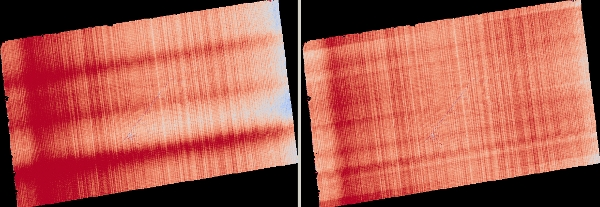
\includegraphics[width=6.0in]{images/jitter.jpg}
\caption{Example of a colorized intersection error map before (left) and
  after jitter correction.}
\label{fig:jitter-example}
\end{figure}


\section{Dealing with Terrain Lacking Large-Scale Features}
\label{sparse-disp}

Stereo Pipeline's approach to performing correlation is a two-step
pyramid algorithm, in which low-resolution versions of the input images
are created, the disparity map
(\texttt{\textit{output\_prefix}-D\_sub.tif}) is found, and then this
disparity map is refined using increasingly higher-resolution versions
of the input images (section \ref{d-sub}).

This approach usually works quite well for rocky terrain but may fail
for snowy landscapes, whose only features may be small-scale
grooves or ridges sculpted by wind (so-called {\it zastrugi}) that
disappear at low resolution.

Stereo Pipeline handles such terrains by using a tool named
\texttt{sparse\_disp} to create
\texttt{\textit{output\_prefix}-D\_sub.tif} at full resolution, yet only
at a sparse set of pixels for reasons of speed. This
low-resolution disparity is then refined as earlier using a pyramid
approach.

\begin{figure}[h!]
\centering
  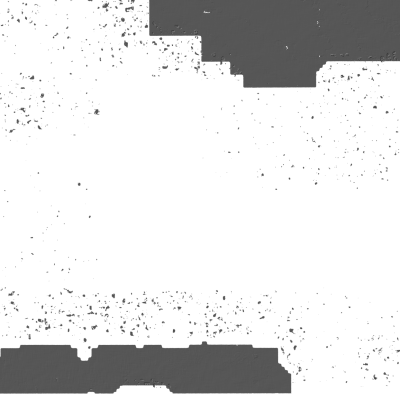
\includegraphics[width=3.0in]{images/examples/sparse_disp1_400px.png}
  
\includegraphics[width=3.0in]{images/examples/sparse_disp3_400px.png}
\caption{Example of a difficult terrain obtained without (left) and with (right) \texttt{sparse\_disp}. (In these DEMs there is very little elevation change, hence the flat appearance.)}
\label{fig:sparse-disp-example}
\end{figure}

This mode can be invoked by passing to \texttt{stereo} the option
\texttt{-\/-corr-seed-mode 3}. Also, during pyramid correlation it is
suggested to use somewhat fewer levels than the default
\texttt{-\/-corr-max-levels 5}, to again not subsample the images too much
and lose the features.

Here is an example:

\begin{verbatim}
    > stereo -t dg --corr-seed-mode 3 --corr-max-levels 2     \
             left_mapped.tif right_mapped.tif                 \
             12FEB12053305-P1BS_R2C1-052783824050_01_P001.XML \
             12FEB12053341-P1BS_R2C1-052783824050_01_P001.XML \
             dg/dg srtm_53_07.tif
\end{verbatim}

If \texttt{sparse\_disp} is not working well for your images you may be
able to improve its results by experimenting with the set of \texttt{sparse\_disp}
options which can be passed into \texttt{stereo} through the 
texttt{-\/-sparse-disp-options} parameter.  \texttt{sparse\_disp}
has so far only been tested with \texttt{affineepipolar} image alignment
so you may not get results with other alignment methods.


Since \texttt{sparse\_disp} is written in Python
it depends on a variety of binary Python modules. These modules cannot
be distributed with Stereo Pipeline as they depend on the version of
Python installed on your system. One way to get these Python modules is
to install them yourself. We reccomend the Conda Python management system
(\href{https://conda.io/docs/index.html}{https://conda.io/docs/index.html})
as an easy way to install these dependencies.

\texttt{sparse\_disp} has been tested on Ubuntu 16.04 using Conda with
following additional packages installed:
\begin{verbatim}
scipy=1.0.0
numpy=1.14.0
simplekml=1.3.0
pyfftw=0.10.4
proj4=4.9.3
gdal=2.2.2
geos=3.6.2
blas=1.0
\end{verbatim}
Note that the \texttt{simplekml} and \texttt{pyfftw} packages needed the argument
\texttt{-c conda-forge} added to their \texttt{conda install} command.

Another way to get these dependencies is to use an installation script
provided by ASP.  It will download and compile the dependencies of
this tool for your platform. The script and instructions are at

\begin{quote}
\indent \href{https://github.com/NeoGeographyToolkit/BinaryBuilder/tree/master/build\_python\_modules}{https://github.com/NeoGeographyToolkit/BinaryBuilder/tree/master/build\_python\_modules}
\end{quote}

After building the \texttt{sparse\_disp} dependencies, per the instructions, the path
to the Python modules must be set, for example as:
\begin{verbatim}
  export ASP_PYTHON_MODULES_PATH=<path to python modules>
\end{verbatim}

This path does not need to be set if you are relying on your own
Python installation such as from Conda.

\section{Processing Multi-Spectral Images}

In addition to panchromatic (grayscale) imagery, the Digital Globe
satellites also produce lower-resolution multi-spectral (multi-band)
images. Stereo Pipeline is designed to process single-band images
only. If invoked on multi-spectral data, it will quietly process the
first band and ignore the rest. To use one of the other
bands it can be singled out by invoking \texttt{dg\_mosaic}
(section \ref{rawdg}) with the \texttt{-\/-band <num>} option. We have
evaluated ASP with Digital Globe's multi-spectral images, but
support for it is still experimental. We recommend using the
panchromatic imagery whenever possible.

\chapter{The Next Steps}
\label{nextsteps}

This chapter will discuss in more detail ASP's stereo process and other
tools available to either pre-process the input images/cameras or to
manipulate \texttt{stereo}'s outputs, both in the context of planetary
ISIS data and for Earth imagery. This includes how to (a) customize
\texttt{stereo}'s settings (b) use \texttt{point2dem} to create 3D
terrain models, (c) visualize the results, (d) align the obtained point
clouds to another data source, (e) perform 3D terrain adjustments in
respect to a geoid, etc.


\section{Stereo Pipeline in More Detail}
\label{running-stereo}

\subsection{Stereo Algorithms}

The default stereo algorithm in ASP is block-matching, with various values for subpixel refinement, as seen below. The latest version of ASP includes the SGM and MGM algorithms, which overall can perform better, but are more experimental. For details about how to invoke these algorithms, see section \ref{sec:sgm}.

\subsection{Setting Options in the \texttt{stereo.default} File}
\label{settingoptionsinstereodefault}

The \texttt{stereo} program requires a \texttt{stereo.default} file that
contains settings that affect the stereo reconstruction process.  Its
contents can be altered for your needs; details are found in appendix
\ref{ch:stereodefault} on page \pageref{ch:stereodefault}.  You may find
it useful to save multiple versions of the \texttt{stereo.default} file
for various processing needs. If you do this, be sure to specify the desired
settings file by invoking \texttt{stereo} with the \texttt{-s}
option.  If this option is not given, the \texttt{stereo} program will
search for a file named \texttt{stereo.default} in the current working
directory. If \texttt{stereo} does not find \texttt{stereo.default} in
the current working directory and no file was given with the \texttt{-s}
option, \texttt{stereo} will assume default settings and continue.

An example \texttt{stereo.default} file is available in the
\texttt{examples/} directory of \ac{ASP}. The actual file has a lot of
comments to show you what options and values are possible. Here's a
trimmed version of the important values in that file.
\begin{verbatim}
        alignment-method affineepipolar
        cost-mode 2
        corr-kernel 21 21
        subpixel-mode 1
        subpixel-kernel 21 21
\end{verbatim}

All these options can be overridden from the command line, as described
in section \ref{cmdline}.

\subsubsection*{Alignment Method}

The most important line in \texttt{stereo.default} is the
first one, specifying the alignment method. For raw images, alignment is
always necessary, as the left and right images are from different
perspectives. Several alignment methods are supported, including
\texttt{affineepipolar} and \texttt{homography} (see section
\ref{stereo-default-preprocessing} for details).

Alternatively, stereo can be performed with map-projected images
(section \ref{mapproj-example}). In effect we take a smooth
low-resolution terrain and map both the left and right raw images onto
that terrain. This automatically brings both images into the same
perspective, and as such, for map-projected images the alignment method
is always set to \texttt{none}.

\subsubsection*{Correlation Parameters}

The second and third lines in \texttt{stereo.default} define what
correlation metric \textit{(normalized cross correlation)} we'll be
using and how big the template or kernel size should be \textit{(21
pixels square)}. A pixel in the left image will be matched to a pixel in
the right image by comparing the windows of this size centered at them.

Making the kernel sizes smaller, such as $15 \times 15$, or even $11
\times 11,$ may improve results on more complex features, such as steep
cliffs, at the expense of perhaps introducing more false matches or
noise.

\subsubsection*{Subpixel Refinement Parameters}

A highly critical parameter in \ac{ASP} is the value of
\texttt{subpixel-mode}, on the fourth line. When set to 1,
\texttt{stereo} performs parabola subpixel refinement, which is very
fast but not very accurate. When set to 2, it produces very accurate
results, but it is about an order of magnitude slower. When set to 3,
the accuracy and speed will be somewhere in between the other methods.

The fifth line sets the kernel size to use during subpixel refinement
\textit{(also 21 pixels square)}.

\subsubsection*{Search Range Determination}

Using these settings alone, \ac{ASP} will attempt to work out the
minimum and maximum disparity it will search for automatically. However if you
wish to, you can explicitly set the extent of the search range by
adding the option:
\begin{verbatim}
        corr-search -80 -2 20 2
\end{verbatim}

More details about this option and the inner workings of stereo correlation
can be found in chapter \ref{ch:correlation}.

\subsection{Performing Stereo Correlation}\label{perform-stereo}

\begin{figure}[t!]
\begin{minipage}{4in}
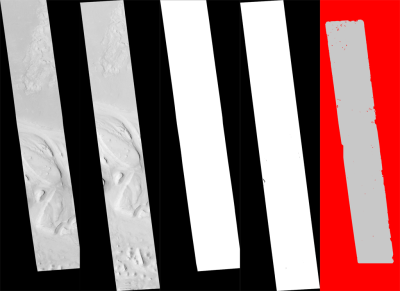
\includegraphics[width=4in]{images/p19-stereo-output_400px.png}
\end{minipage}
\hfill
\begin{minipage}{2.9in}
\caption[P19 stereo output images]{
    \label{p19-stereo-output}
        These are the four viewable \texttt{.tif} files created by the
        \texttt{stereo} program.  On the left are the two aligned,
        pre-processed images: (\texttt{results/output-L.tif} and
        \texttt{results/output-R.tif}).  The next two are mask images
        (\texttt{results/output-lMask.tif} and
        \texttt{results/output-rMask.tif}), which indicate which
        pixels in the aligned images are good to use in stereo
        correlation.  The image on the right is the ``Good Pixel
        map'', (\texttt{results/output-GoodPixelMap.tif}), which
        indicates (in gray) which were successfully matched with the
        correlator, and (in red) those that were not matched.}
\end{minipage}
\end{figure}

As already mentioned, the \texttt{stereo} program can be invoked for ISIS
images as

\begin{verbatim}
  ISIS 3> stereo left_image.cub right_image.cub \
            -s stereo.default results/output
\end{verbatim}

For Digital Globe imagery the cameras need to be specified separately:


\begin{verbatim}
  > stereo left.tif right.tif left.xml right.xml \
      -s stereo.default results/output
\end{verbatim}

As stated in section \ref{quickstart}, the string
\texttt{results/output} is arbitrary, and in this case we will
simply make all outputs go to the \texttt{results} directory.

When \texttt{stereo} finishes, it will have produced a point cloud
image. Section \ref{visualising} describes how to convert it to a
digital elevation model (DEM) or other formats.

The \texttt{stereo} command can also take multiple input images, performing
multi-view stereo (section \ref{multiview}).

\subsection{Running the GUI Frontend}
The \texttt{stereo\_gui} program is a GUI frontend to \texttt{stereo}.
It is invoked with the same options as \texttt{stereo}. It displays
the input images, and makes it possible to zoom in and select smaller
regions to run stereo on. The GUI is described in section \ref{stereo_gui}.

\subsection{Specifying Settings on the Command Line}
\label{cmdline}

All the settings given via the \texttt{stereo.default} file can be
over-ridden from the command line. Just add a double hyphen
(\texttt{-\/-}) in front the option's name and then fill out the option
just as you would in the configuration file. For options in the
\texttt{stereo.default} file that take multiple numbers, they must be
separated by spaces (like `\texttt{corr-kernel~25~25}') on the command
line. Here is an example in which we override the search range and
subpixel mode from the command line.

\begin{verbatim}
  ISIS 3> stereo E0201461.map.cub M0100115.map.cub  \
            -s stereo.map --corr-search -70 -4 40 4 \
            --subpixel-mode 0 results/output
\end{verbatim}

\subsection{Stereo on Multiple Machines}

If the input images are really large it may desirable to distribute the
work over several computing nodes. ASP provides a tool named
\texttt{parallel\_stereo} for that purpose. Its usage is described in section
\ref{parallel}.

\subsection{Running Stereo with Map-projected Images}
\label{mapproj-example}

The way stereo correlation works is by matching a neighborhood of each
pixel in the left image to a similar neighborhood in the right image.
This matching process can fail or become unreliable if the two images
are too different, which can happen for example if the perspectives
of the two cameras are very different or the underlying terrain has
steep portions. This will result in ASP producing terrains with noise or
missing data.

ASP can mitigate this by \textit{map-projecting} the left and right
images onto some pre-existing low-resolution smooth terrain model
without holes, and using the output images to do stereo. In effect, this
makes the images much more similar and more likely for stereo
correlation to succeed.

In this mode, ASP does not create a terrain model from scratch,
but rather uses an existing terrain model as an initial guess, and
improves on it.

For Earth, an existing terrain model can be, for example, NASA SRTM,
GMTED2010, USGS's NED data, or NGA's DTED data. There exist pre-made
terrain models for other planets as well, for example the Moon LRO LOLA
global DEM and the Mars MGS MOLA DEM.


Alternatively, a low-resolution smooth DEM can be obtained by running
ASP itself as described in previous sections. In such a run, subpixel
mode may be set to parabola (\texttt{subpixel-mode 1}) for speed. To
make it sufficiently coarse and smooth, the resolution can be set to
about 40 times coarser than either the default \texttt{point2dem}
resolution or the resolution of the input images. If the resulting DEM
turns out to be noisy or have holes, one could change in
\texttt{point2dem} the search radius factor, use hole-filling, invoke more
aggressive outlier removal, and erode pixels at the boundary (those
tend to be less reliable). Alternatively, holes can be filled with
\texttt{dem\_mosaic}.

The tool used for map-projecting the images is called
\texttt{mapproject} (section \ref{mapproject}). It is very important to
specify correctly the output resolution (the \texttt{-\/-tr} option for
\texttt{mapproject}) when creating map-projected images. For example, if
the input images are about 1 meter/pixel, the same number should be used
in \texttt{mapproject} (if the desired projection is in degrees, this
value should be converted to degrees). If the output resolution is not
correct, there will be artifacts in the stereo results.

Some experimentation on a small area may be necessary to obtain the best
results. Once images are map-projected, they can be cropped to a small
shared region using \texttt{gdal\_translate -projwin} and then 
stereo with these clips can be invoked. 

\subsubsection{Example for ISIS images}

\begin{figure}[h!]
\centering
   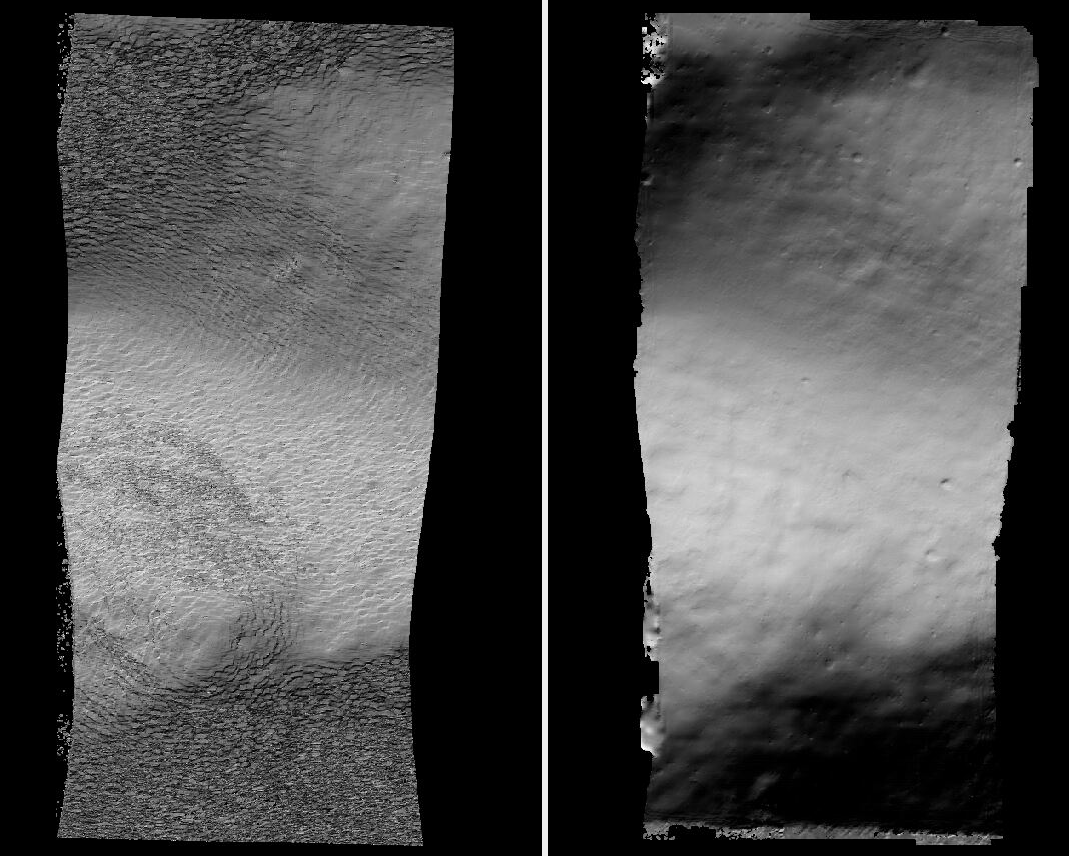
\includegraphics[width=6.0in]{images/stereo_mapproj_400px.png}
\caption{A DEM obtained using plain stereo (left) and stereo
  with map-projected images (right). Their quality will be comparable
  for relatively flat terrain and the second will be much better for
  rugged terrain. The right image has some artifacts, but those are limited
  to areas close to the boundary.}
\label{fig:mapproj-example}
\end{figure}

In this example we illustrate how to run stereo with map-projected
images for ISIS data. We start with LRO NAC Lunar images M1121224102LE
and M1121209902LE from ASU's LRO NAC web site,
http://lroc.sese.asu.edu/. We convert them to ISIS cubes using the ISIS
program \texttt{lronac2isis}, then we use the ISIS tools
\texttt{spiceinit}, \texttt{lronaccal}, and \texttt{lrnonacecho} to
update the SPICE kernels and to do radiometric and echo correction. We
name the two obtained .cub files \texttt{left.cub} and
\texttt{right.cub}.

Here we decided to run ASP to create the low-resolution DEM needed for
map-projection, rather than get them from an external source. For speed,
we process just a small portion of the images:

\begin{verbatim}
  parallel_stereo left.cub right.cub            \
    --left-image-crop-win 1984 11602 4000 5000  \
    --right-image-crop-win 3111 11027 4000 5000 \
    --job-size-w 1024 --job-size-h 1024         \
    --subpixel-mode 1                           \
    run_nomap/run
\end{verbatim}

(the crop windows can be determined using \texttt{stereo\_gui}). 
The input images have resolution of about 1 meter, or $3.3 \times
10^{-5}$ degrees on the Moon. We create the low-resolution DEM using a
resolution 40 times as coarse, so we use a grid size of $0.0013$ degrees
(we use degrees since the default \texttt{point2dem} projection invoked
here is \texttt{longlat}).

\begin{verbatim}
  point2dem --search-radius-factor 5 --tr 0.0013 run_nomap/run-PC.tif 
\end{verbatim}

As mentioned earlier, some tweaks to the parameters used by \texttt{point2dem}
may be necessary for this low-resolution DEM to be smooth enough and
with no holes.

Note that we used \texttt{-\/-search-radius-factor 5} to expand the DEM
a bit, to counteract future erosion in stereo due to the correlation kernel
size.

If this terrain is close to the poles, say within 25 degrees of
latitude, it is advised to use a stereographic projection, centered
either at the nearest pole, or close to the center of the current
DEM. Its center's longitude and latitude can be found with
\texttt{gdalinfo -stats}, which can then be passed to \texttt{point2dem}
such as

\begin{verbatim}
  point2dem --stereographic --proj-lon <lon_ctr> --proj-lat <lat_ctr> ...
\end{verbatim}

By calling \texttt{gdalinfo -proj4}, the PROJ.4 string of the obtained DEM can
be found, which can be used in mapprojection later, and with the resolution
switched to meters from degrees (see section \ref{dg-mapproj} for more details). 

Next, we map-project the images onto this DEM, using the original resolution
of $3.3 \times 10^{-5}$ degrees.

\begin{verbatim}
  mapproject --tr 0.000033 run_nomap/run-DEM.tif left.cub left_proj.tif \
    --t_projwin 3.6175120 25.5669989 3.6653695 25.4952127
  mapproject --tr 0.000033 run_nomap/run-DEM.tif right.cub right_proj.tif \
    --t_projwin 3.6175120 25.5669989 3.6653695 25.4952127
\end{verbatim}

Notice that we restricted the area of computation using \texttt{-\/-t\_projwin}
to again make the process faster.

Next, we do stereo with these map-projected images.

\begin{verbatim}
  parallel_stereo --job-size-w 1024 --job-size-h 1024 \
    --subpixel-mode 3                                 \
    left_proj.tif right_proj.tif left.cub right.cub   \
    run_map/run run_nomap/run-DEM.tif
\end{verbatim}

Notice that even though we use map-projected images, we still specified
the original images as the third and fourth arguments. That because we
need the camera information from those files.  The fifth argument is
the output prefix, while the sixth is the low-resolution DEM we used for
map-projection. We have used here \texttt{-\/-subpixel-mode 3} as this
will be the final point cloud and we want the increased accuracy.

Lastly, we create a DEM at 1 meter resolution:
\begin{verbatim}
  point2dem --nodata-value -32768 --tr 0.000033 run_map/run-PC.tif
\end{verbatim}
Note here that we could have used a coarser resolution for the final
DEM, such as 4 meters/pixel, since we won't see detail at the level of
1 meter in this DEM, as the stereo process is lossy. This is
explained in more detail in section \ref{post-spacing}.

In figure \ref{fig:mapproj-example} we show the effect of using
map-projected images on accuracy of the final DEM.

It is important to note that we could have map-projected the images
using the ISIS tool \texttt{cam2map}, as described in section
\ref{sec:AligningImages}. The current approach could be preferable since
it allows us to choose the DEM to map-project onto, and it is much faster,
since ASP's \texttt{mapproject} uses multiple processes, while \texttt{cam2map}
is restricted to one process and one thread.

\subsubsection{Example for Digital Globe Images}
\label{dg-mapproj}

In this section we will describe how to run stereo with map-projected
images for Digital Globe cameras for Earth. The same process can be used
with very minor modifications for any satellite imagery that uses the
the RPC camera model. All that is needed is to replace the stereo
session when invoking \texttt{stereo} below with \texttt{rpcmaprpc} from
\texttt{dgmaprpc}.

Unlike the previous section, here we will use an external DEM to map-project
onto, rather than creating our own. We will use a variant of NASA
SRTM data with no holes. Other choices have been mentioned earlier.

It is important to note that ASP expects the input low-resolution DEM to
be in reference to a datum ellipsoid, such as WGS84 or NAD83. If the DEM
is in respect to either the EGM96 or NAVD88 geoids, the ASP tool
\texttt{dem\_geoid} can be used to convert the DEM to WGS84 or NAD83
(section \ref{demgeoid}). (The same tool can be used to convert back the
final output ASP DEM to be in reference to a geoid, if desired.)

Not applying this conversion might not properly negate the parallax
seen between the two images, though it will not corrupt the
triangulation results. In other words, sometimes one may be able to
ignore the vertical datums on the input but we do not recommend
doing that. Also, you should note that the geoheader attached to those
types of files usually does not describe the vertical datum they
used. That can only be understood by careful reading of your
provider's documents.

In this example we use as an input low-resolution DEM the file
\texttt{srtm\_53\_07.tif}, a 90 meter resolution tile from the CGIAR-CSI
modification of the original NASA SRTM product \cite{cgiar:srtm90m}.
The NASA SRTM square for this example spot in India is N26E080.

Below are the commands for map-projecting the input and then running
through stereo. You can use any projection you like as long as it
preserves detail in the imagery. Note that the last parameter in the
stereo call is the input low-resolution DEM. The dataset is the same
as the one used in section \ref{rawdg}.

\begin{figure}[h!]
\centering
  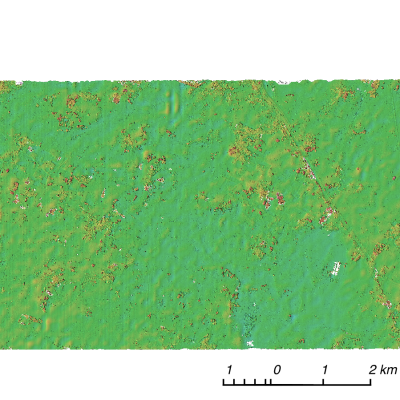
\includegraphics[width=2.0in]{images/examples/dg/MappedContext_400px.png}
  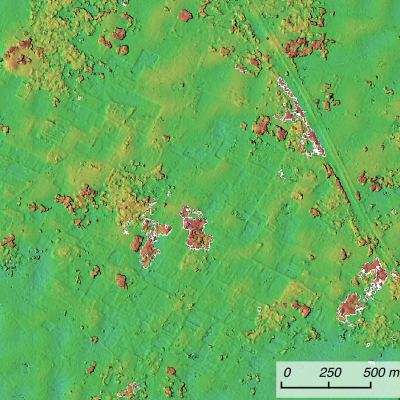
\includegraphics[width=2.0in]{images/examples/dg/MappedCloseUp_400px.png}
  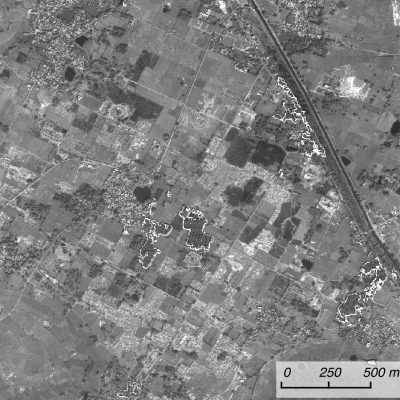
\includegraphics[width=2.0in]{images/examples/dg/MappedCloseUpDRG_400px.png}
\caption{Example colorized height map and ortho image output.}
\label{fig:dg-map-example}
\end{figure}

\subsubsection*{Commands}

\begin{verbatim}
    mapproject -t rpc --t_srs "+proj=eqc +units=m +datum=WGS84" \
      --tr 0.5 srtm_53_07.tif                            \
      12FEB12053305-P1BS_R2C1-052783824050_01_P001.TIF   \
      12FEB12053305-P1BS_R2C1-052783824050_01_P001.XML   \
      left_mapped.tif
    mapproject -t rpc --t_srs "+proj=eqc +units=m +datum=WGS84" \
      --tr 0.5 srtm_53_07.tif                            \
      12FEB12053341-P1BS_R2C1-052783824050_01_P001.TIF   \
      12FEB12053341-P1BS_R2C1-052783824050_01_P001.XML   \
      right_mapped.tif
    stereo -t dgmaprpc --subpixel-mode 1 --alignment-method none  \
           left_mapped.tif right_mapped.tif                 \
           12FEB12053305-P1BS_R2C1-052783824050_01_P001.XML \
           12FEB12053341-P1BS_R2C1-052783824050_01_P001.XML \
           dg/dg srtm_53_07.tif
\end{verbatim}

If the \texttt{-\/-t\_srs} option is not specified, it will be read from
the low-resolution input DEM.

The complete list of options for \texttt{mapproject} is described in
section \ref{mapproject}.

In the \texttt{stereo} command, we have used \texttt{subpixel-mode 1}
which is less accurate but reasonably fast. We have also used
\texttt{alignment-method none}, since the images are map-projected onto
the same terrain with the same resolution, thus no additional alignment
is necessary. More details about how to set these and other
\texttt{stereo} parameters can be found in section
\ref{settingoptionsinstereodefault}.

It is important to note here that any Digital Globe camera file has two
models in it, the exact linescan model (which we name \texttt{DG}), and
its \texttt{RPC} approximation. Above, we have used the approximate RPC
model for map-projection, since map-projection is just a pre-processing
step to make the images more similar to each other, this step will be
undone during stereo triangulation, and hence using the RPC model is
good enough, while being much faster than the exact \texttt{DG}
model. At the stereo stage, we see above that we invoked the
\texttt{dgmaprpc} session, which suggests that we have used the RPC
model during map-projection, but we would like to use the accurate DG
model when performing actual triangulation from the cameras to the
ground.

\subsubsection{RPC and Pinhole Camera Models}

Map-projected images can also be used with RPC and Pinhole camera
models. The \texttt{mapproject} command needs to be invoked with
\texttt{-t rpc} and \texttt{-t pinhole} respectively. As earlier, when
invoking \texttt{stereo} the the first two arguments should be the
map-projected images, followed by the camera models, output prefix, and
the name of the DEM used for map-projection. The session name passed to
\texttt{stereo} should be \texttt{rpcmaprpc} and
\texttt{pinholemappinhole} respectively.

\subsection{Multi-View Stereo}
\label{multiview}

ASP supports multi-view stereo at the triangulation stage.  In this
scenario, the first image is set as reference, disparities are
computed from it to all the other images, and then joint triangulation
is performed \cite{slabaugh2001optimal}. A single
point cloud is generated with one 3D point for each pixel in the first
image. The inputs to multi-view stereo and its output point cloud are
handled in the same way as for two-view stereo (e.g., inputs can be
map-projected, the output can be converted to a DEM, etc.).

It is suggested that images be bundle-adjusted (section section
\ref{baasp}) before running multi-view stereo.

Example (for ISIS with three images):
\begin{verbatim}
  stereo file1.cub file2.cub file3.cub results/run
\end{verbatim}

Example (for Digital Globe data with three map-projected images):
\begin{verbatim}
  stereo file1.tif file2.tif file3.tif file1.xml file2.xml file3.xml \
    results/run input-DEM.tif
\end{verbatim}

The \texttt{parallel\_stereo} tool can also be used with multiple images
(section \ref{parallel}).

For a sequence of images, multi-view stereo can be run several times
with each image as a reference, and the obtained point clouds combined
into a single DEM using \texttt{point2dem} (section \ref{point2dem}).

The ray intersection error, the fourth band in the point cloud
file, is computed as twice the mean of distances from the optimally
computed intersection point to the individual rays. For two rays, this
agrees with the intersection error for two-view stereo which is defined
as the minimal distance between rays. For multi-view stereo this error
is much less amenable to interpretation than for two-view stereo, since the
number of valid rays corresponding to a given feature can vary across
the image, which results in discontinuities in the intersection error.

\subsubsection*{Other ways of combining multiple images}

As an alternative to multi-view stereo, point clouds can be generated
from multiple stereo pairs, and then a single DEM can be created with
\texttt{point2dem} (section \ref{builddem}). Or, multiple DEMs
can be created, then combined into a single DEM with \texttt{dem\_mosaic}
(section \ref{demmosaic}).

In both of these approaches, the point clouds could be registered
to a trusted dataset using \texttt{pc\_align} before creating a combined
terrain model (section \ref{pc-align-example}).

The advantage of creating separate DEMs and then merging them (after
alignment) with \texttt{dem\_mosaic}, compared to multivew trianglation,
is that this approach will not create visible seams, while likely it will
still increase the accuracy compared to the individual input DEMs.

\subsection{Diagnosing Problems}

Once invoked, \texttt{stereo} proceeds through several stages that are
detailed on page \pageref{entrypoints}.  Intermediate and final output
files are generated as it goes.  See Appendix
\ref{chapter:outputfiles}, page \pageref{chapter:outputfiles} for a
comprehensive listing.  Many of these files are useful for diagnosing and
debugging problems.  For example, as Figure~\ref{p19-stereo-output}
shows, a quick look at some of the TIFF files in the \texttt{results/}
directory provides some insight into the process.

Perhaps the most accessible file for assessing the quality of your
results is the good pixel image, \\
(\texttt{results/output-GoodPixelMap.tif}).  If this file shows mostly
good, gray pixels in the overlap area (the area that is white in both
the \texttt{results/output-lMask.tif} and
\texttt{results/output-rMask.tif} files), then your results are just
fine.  If the good pixel image shows lots of failed data, signified by
red pixels in the overlap area, then you need to go back and tune your
\texttt{stereo.default} file until your results improve.  This might be
a good time to make a copy of \texttt{stereo.default} as you tune the
parameters to improve the results.

\begin{figure}[b!]
\begin{minipage}{4in}
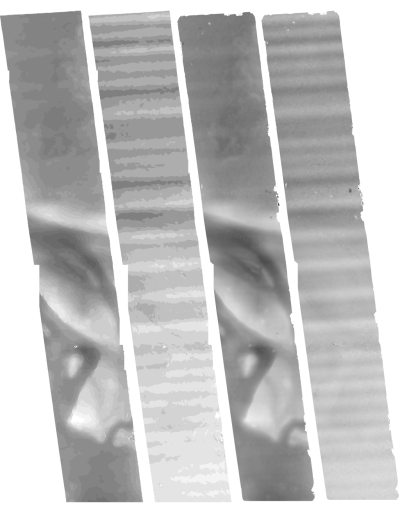
\includegraphics[width=4in]{images/p19-disparity_400px.png}
\end{minipage}
\hfill
\begin{minipage}{2.7in}
\caption[P19 disparity images]{
    \label{p19-disparity}
	Disparity images produced using the \texttt{disparitydebug}
        tool.  The two images on the left are the
        \texttt{results/output-D-H.tif} and
        \texttt{results/output-D-V.tif} files, which are normalized
        horizontal and vertical disparity components produced by the
        disparity map initialization phase.  The two images on the
        right are \texttt{results/output-F-H.tif} and
        \texttt{results/output-F-V.tif}, which are the final
        filtered, sub-pixel-refined disparity maps that are fed into the
        Triangulation phase to build the point cloud image.  Since
        these MOC images were acquired by rolling the spacecraft
        across-track, most of the disparity that represents topography
        is present in the horizontal disparity map.  The vertical
        disparity map shows disparity due to ``wash-boarding,'' which
        is not from topography but from spacecraft movement. Note
        however that the horizontal and vertical disparity images are
        normalized independently.  Although both have the same range
        of gray values from white to black, they represent
        significantly different absolute ranges of disparity.}
\end{minipage}
\end{figure}

Whenever \texttt{stereo}, \texttt{point2dem}, and other executables are
run, they create log files in given tool's results directory, containing
a copy of the configuration file, the command that was run, your system
settings, and tool's console output. This will help track what was
performed so that others in the future can recreate your work.

Another handy debugging tool is the \texttt{disparitydebug} program,
which allows you to generate viewable versions of the intermediate
results from the stereo correlation algorithm.
\texttt{disparitydebug} converts information in the disparity image
files into two TIFF images that contain horizontal and vertical
components of the disparity (i.e. matching offsets for each pixel in
the horizontal and vertical directions).  There are actually three
flavors of disparity map: the \texttt{-D.tif}, the \texttt{-RD.tif},
and \texttt{-F.tif}.  You can run \texttt{disparitydebug} on any of
them.  Each shows the disparity map at the different stages of
processing.

\begin{verbatim}
  >  disparitydebug results/output-F.tif
\end{verbatim}

If the output H and V files from \texttt{disparitydebug} look good,
then the point cloud image is most likely ready for post-processing.
You can proceed to make a mesh or a \ac{DEM} by processing
\texttt{results/output-PC.tif} using the \texttt{point2mesh} or
\texttt{point2dem} tools, respectively.

Figure \ref {p19-disparity} shows the outputs of \texttt{disparitydebug}.

If the input images are map-projected (georeferenced) and the alignment
method is \texttt{none}, all images output by stereo are georeferenced
as well, such as GoodPixelMap, D\_sub, disparity, etc. As such, all
these data can be overlayed in
\texttt{stereo\_gui}. \texttt{disparitydebug} also preserves any
georeference.

\subsection{Dealing with Long Run-times}
\label{longrun}

If \texttt{stereo\_corr} takes unreasonably
long, it may have encountered a portion of the image where, due to noise
(such as clouds, shadows, etc.) the determined search range is much
larger than what it should be. The option \texttt{-\/-corr-timeout \textit{integer}}
can be used to limit how long each 1024$\times$1024 pixel tile can take.
A good value here could be 300 (seconds) or more if your terrain is expected
to have large height variations.

\section{Visualizing and Manipulating the Results}
\label{visualising}

When \texttt{stereo} finishes, it will have produced a point cloud
image.  At this point, many kinds of data products can be built from
the \texttt{results/output-PC.tif} point cloud file.

\begin{figure}[h!]
\begin{minipage}{5in}
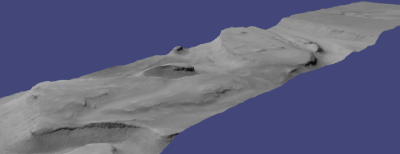
\includegraphics[width=5in]{images/p19-osg_400px.png}
\end{minipage}
\hfill
\begin{minipage}{1.7in}
\caption[P19 in OSG]{
    \label{p19-osg}
	The \texttt{results/output.osgb} file displayed in the OSG
        Viewer.}
\end{minipage}
\end{figure}

\subsection{Building a 3D Mesh Model}
If you wish to see the data in an interactive 3D browser, then you can
generate a 3D object file using the \texttt{point2mesh} command (page
\pageref{point2mesh}). The resulting file is stored in Open Scene
Graph binary format \cite{OSG_website}.  It can be viewed with
\texttt{osgviewer} (the Open Scene Graph Viewer program, distributed
with the binary version of the Stereo Pipeline).  The
\texttt{point2mesh} program takes the point cloud file and the left
normalized image as inputs:

\begin{verbatim}
  > point2mesh results/output-PC.tif results/output-L.tif
  > osgviewer results/output.osgb
\end{verbatim}

The image displayed by \texttt{osgviewer} is shown in figure \ref{p19-osg}.

When the \texttt{osgviewer} program starts, you may want to toggle the
lighting with the `L' key, toggle texturing with the 'T' key, and
toggle wireframe mode with the 'W'.  Press '?' to see a variety of
other interactive options.

If you already have a DEM and an ortho image (section \ref{builddem}),
they can be used to build a mesh as well, in the same way as done above:
\begin{verbatim}
  > point2mesh results/output-DEM.tif results/output-DRG.tif
\end{verbatim}

\subsection{Building a Digital Elevation Model and Ortho Image}
\label{builddem}

The \texttt{point2dem} program (page \pageref{point2dem}) creates a
Digital Elevation Model (\ac{DEM}) from the point cloud file.

\begin{verbatim}
  >  point2dem results/output-PC.tif
\end{verbatim}

The resulting TIFF file is map-projected and will contain
georeferencing information stored as GeoTIFF tags.

The tool will infer the datum and projection from the input images, if
present. You can explicitly specify a coordinate system (e.g.,
mercator, sinusoidal) and a reference spheroid (i.e., calculated for the
Moon, Mars, or Earth). Alternatively, the datum semi-axes can be set or
a PROJ.4 string can be passed in.

\begin{verbatim}
  >  point2dem -r mars results/output-PC.tif
\end{verbatim}

The output DEM will be named \texttt{results/output-DEM.tif}.
It can be imported into a variety of GIS platforms.
The DEM can be transformed into a hill-shaded image for visualization
(section \ref{genhillshade}). Both the DEM itself and its hill-shaded
version can be examined in \texttt{stereo\_gui}.

The \texttt{point2dem} program can also be used to orthoproject raw
satellite imagery onto the \ac{DEM}. To do this, invoke
\texttt{point2dem} just as before, but add the \texttt{-\/-orthoimage}
option and specify the use of the left image file as the texture file
to use for the projection:

\begin{verbatim}
  >  point2dem results/output-PC.tif --orthoimage results/output-L.tif
\end{verbatim}

The texture file must always be specified after the point cloud file in
this command. See figure \ref{p19-norm_ortho} on the right for the
output image.

To fill in any holes in the obtained orthoimage, one can invoke it
with a larger value of the grid size (the \texttt{-\/-tr} option)
and/or with a variation of the options:

\begin{verbatim}
   --no-dem --orthoimage-hole-fill-len 100 --search-radius-factor 2 
\end{verbatim}

The \texttt{point2dem} program is also able to accept output
projection options the same way as the tools in GDAL. Well-known EPSG,
IAU2000 projections, and custom PROJ.4 strings can applied with the
target spatial reference set flag, \texttt{-\/-t\_srs}. If the target
spatial reference flag is applied with any of the reference spheroid
options, the reference spheroid option will overwrite the datum
defined in the target spatial reference set. The following examples
produce the same output. However, the last two results will also 
show correctly the name of the datum in the geoheader, not just the values
of its axes.

\begin {verbatim}
  point2dem --t_srs "+proj=longlat +a=3396190 +b=3376200"
     results/output-PC.tif

  point2dem --t_srs http://spatialreference.org/ref/iau2000/49900/ \
     results/output-PC.tif

   point2dem --t_srs 'GEOGCS["Geographic Coordinate System",                     
                         DATUM["D_Mars_2000",
                         SPHEROID["Mars_2000_IAU_IAG",3396190,169.894447223611]],
                         PRIMEM["Greenwich",0],
                         UNIT["degree",0.0174532925199433]]' results/output-PC.tif
\end{verbatim}

The \texttt{point2dem} program can be used in many different ways. The
complete documentation is in section \ref{point2dem}.

\begin{figure}
\hfill
\begin{minipage}{3.5in}
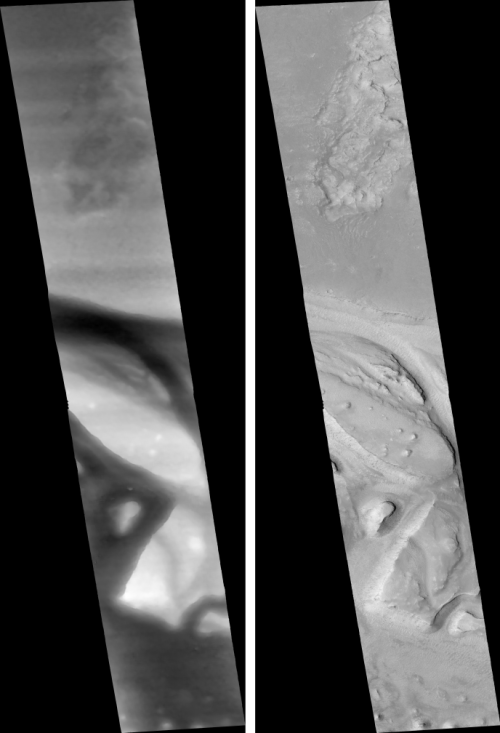
\includegraphics[width=3.5in]{images/p19-norm_ortho_500px.png}
\end{minipage}
\hfill
\begin{minipage}{2in}
\caption[P19 Normalized DEM and Orthophoto]{
    \label{p19-norm_ortho}
	The image on the left is a normalized DEM (generated using
        \texttt{point2dem}'s
        \texttt{-n} option), which shows low terrain values as black
        and high terrain values as white.  The image on the right is
        the left input image projected onto the DEM (created using the
        \texttt{-\/-orthoimage} option to \texttt{point2dem}).  }
\end{minipage}
\hfill
\end{figure}

\subsection{Orthorectification of an Image From a Different Source}
If you have already obtained a DEM, using ASP or some other approach, and have
an image and camera pair which you would like to overlay on top of this terrain,
use the \texttt{mapproject} tool (section \ref{mapproject}).


% \begin{figure}
% \begin{center}
% \includegraphics[width=4in]{images/p19-dems.png}
% \caption[P19 dem images]{
%     \label{p19-dems}
%	The non-normalized and normalized DEMs. Note that the
%	non-normalized version contains floating point pixel values
%	and will not open in most image viewing programs which
%	expect integer pixel values between 0 and 255 (which is
%	what the normalized version does for you).
%     }
% \end{center}
% \end{figure}
%
% \begin{figure}
% \begin{center}
% \includegraphics[width=3in]{images/p19-ortho.png}
% \caption[P19 orthophoto]{
%     \label{p19-ortho}
%	The left image orthoprojected onto the DEM.
%     }
% \end{center}
% \end{figure}

\newpage

\subsection{Correcting Camera Positions and Orientations}

The \texttt{bundle\_adjust} program can be used to adjust the camera
positions and orientations before running stereo. These adjustments only
makes the cameras self-consistent. For the adjustments to be absolute,
it is necessary to use \texttt{bundle\_adjust} with ground control
points. This tool is described in section \ref{bundleadjust}.

\subsection{Alignment to Point Clouds From a Different Source}
\label{pc-align-example}
Often the 3D terrain models output by \texttt{stereo} (point
clouds and DEMs) can be intrinsically quite accurate yet their actual
position on the planet may be off by several meters or several
kilometers, depending on the spacecraft. This can result from small
errors in the position and orientation of the satellite cameras taking
the pictures.

Such errors can be corrected in advance using bundle adjustment, as
described in the previous section. That requires using ground control
points, that may not be easy to collect. Alliteratively, the images and
cameras can be used as they are, and the absolute position of the output
point clouds can be corrected in post-processing. For that, ASP provides
a tool named \texttt{pc\_align}. It aligns a 3D terrain to a much more
accurately positioned (if potentially sparser) dataset. Such datasets
can be made up of GPS measurements (in the case of Earth), or from
laser altimetry instruments on satellites, such as ICESat/GLASS for
Earth, LRO/LOLA on the Moon, and MGS/MOLA on Mars.  Under the hood,
\texttt{pc\_align} uses the Iterative Closest Point algorithm (ICP)
(both the point-to-plane and point-to-point flavors are supported,
and with point-to-point ICP it is also possible to solve for a scale change).

The \texttt{pc\_align} tool requires another input, an a priori guess for
the maximum displacement we expect to see as result of alignment, i.e.,
by how much the points are allowed to move when the alignment transform is
applied. If not known, a large (but not unreasonably so) number can be
specified. It is used to remove most of the points in the source
(movable) point cloud which have no chance of having a corresponding
point in the reference (fixed) point cloud.

Here is how \texttt{pc\_align} can be called (the denser cloud is
specified first).

\begin{figure}
\hfill
\begin{minipage}{3.5in}
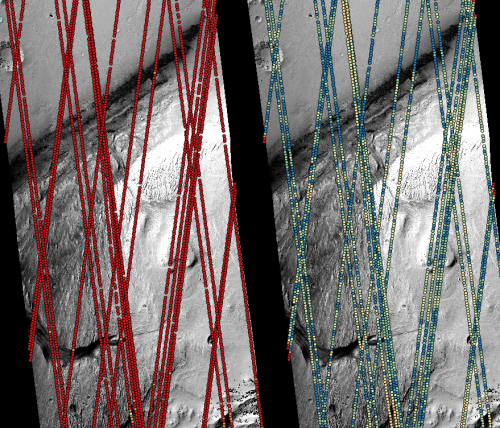
\includegraphics[width=2.5in]{images/examples/align_compare_500px.png}
\end{minipage}
\hfill
\begin{minipage}{2in}
\caption[pc-align comparison]{
Example of using \texttt{pc\_align} to align a DEM obtained using stereo
from CTX images to a set of MOLA tracks. The MOLA points are colored by the offset error
initially (left) and after pc align was applied (right)
to the terrain model. The red dots indicate
more than 100 m of error and blue less than 5 m. The
\texttt{pc\_align} algorithm determined that by moving the terrain
model approximately 40 m south, 70 m west, and
175 m vertically, goodness of
fit between MOLA and the CTX model was increased substantially.
}
\label{pc-align-fig}
\end{minipage}
\hfill
\end{figure}

\begin {verbatim}
  >  pc_align --max-displacement 200 --datum MOLA   \
       --save-inv-transformed-reference-points      \
       --csv-format '1:lon 2:lat 3:radius_m'        \
       stereo-PC.tif mola.csv
\end{verbatim}

It is important to note here that there are two widely used Mars datums,
and if your CSV file has, unlike above, the heights relative to a datum,
the correct datum name must be specified via \texttt{-\/-datum}. Section
\ref{molacmp} talks in more detail about the Mars datums.

Figure \ref{pc-align-fig} shows an example of using \texttt{pc\_align}.
The complete documentation for this program is in section
\ref{pcalign}.

\subsection{Alignment and Orthoimages}

Two related issues are discussed here. The first is that sometimes, after ASP has created
a DEM, and the left and right images are map-projected to it, they are shifted in respect to 
each other. That is due to the errors in camera positions. To rectify it, one has to
run \texttt{bundle\_adjust} first, then rerun the stereo and mapprojection tools, with the
adjusted cameras being passed to both via \texttt{-\/-bundle-adjust-prefix}. 

Note that this approach will create self-consistent outputs, but not necessarily aligned
with pre-existing ground truth. That we deal with next. 

Once an ASP-generated DEM has been aligned to known ground data using
\texttt{pc\_align}, it may be desired to create orthoimages that are
also aligned to the ground. That can be accomplished in two ways.

The \texttt{point2dem -\/-orthoimage} approach be used, and one can pass
to it the point cloud after alignment and the \texttt{L} image before alignment
(all this tool does is copy pixels from the texture image, so position errors are not a problem).

Alternatively, one can invoke the \texttt{mapproject} tool again. Yet, there is a challenge,
because this tool uses the original cameras, before alignment, but will project onto the
DEM after alignment, so the obtained orthoimage location on the ground will be wrong. 

The solution is to invoke \texttt{bundle\_adjust} on the two input images and cameras, while passing
to it the transform obtained from \texttt{pc\_align} via the \texttt{-\/-initial-transform}
option. This will shift the cameras to the right place, and then \texttt{mapproject}
can be called with the adjusted cameras, using again the \texttt{-\/-bundle-adjust-prefix}
option. If all that is wanted is to shift the cameras, without doing any actual adjustments,
the tool can be invoked with 0 iterations. 

\subsection{Creating DEMs Relative to the Geoid/Areoid}

The DEMs generated using \texttt{point2dem} are in reference to a datum
ellipsoid. If desired, the \texttt{dem\_geoid} program can be used to
convert this DEM to be relative to a geoid/areoid on Earth/Mars
respectively. Example usage:

\begin {verbatim}
  >  dem_geoid results/output-DEM.tif
\end{verbatim}

\subsection{Converting to the LAS Format}

If it is desired to use the \texttt{stereo} generated point cloud
outside of ASP, it can be converted to the LAS file format, which is a public file
format for the interchange of 3-dimensional point cloud data. The tool
\texttt{point2las} can be used for that purpose (section
\ref{point2las}). Example usage:

\begin {verbatim}
  >  point2las --compressed -r Earth results/output-PC.tif
\end{verbatim}

\subsection{Generating Color Hillshade Maps}
\label{genhillshade}

Once you have generated a \ac{DEM} file, you can use the
\texttt{colormap} and \texttt{hillshade} tools to create colorized
and/or shaded relief images.

To create a colorized version of the \ac{DEM}, you need only specify
the \ac{DEM} file to use. The colormap is applied to the full range of
the DEM, which is computed automatically.  Alternatively you can
specify your own min and max range for the color map.

\begin{verbatim}
  >  colormap results/output-DEM.tif -o hrad-colorized.tif
\end{verbatim}

To create a hillshade of the \ac{DEM}, specify the \ac{DEM} file to
use. You can control the azimuth and elevation of the light source
using the \texttt{-a} and \texttt{-e} options.

\begin{verbatim}
  >  hillshade results/output-DEM.tif -o hrad-shaded.tif -e 25 -a 300
\end{verbatim}

To create a colorized version of the shaded relief file, specify
the \ac{DEM} and the shaded relief file that should be used:

\begin{verbatim}
  >  colormap results/output-DEM.tif -s hrad-shaded.tif -o hrad-color-shaded.tif
\end{verbatim}

See figure \ref{hrad-color} showing the images obtained with these commands.

The complete documentation for \texttt{colormap} is in section
\ref{sec:colormap}, and for \texttt{hillshade} in section \ref{sec:hillshade}.

\begin{figure}[b!]
\begin{center}
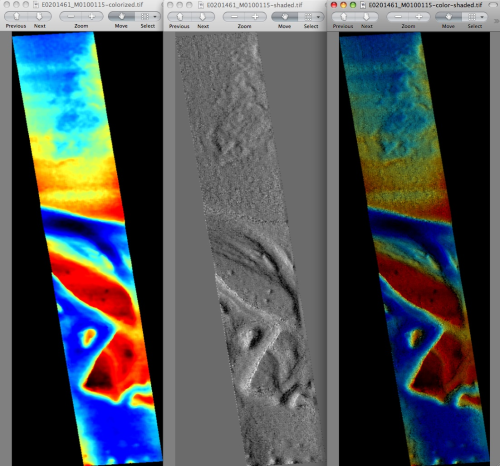
\includegraphics[width=4.7in]{images/p19-colorized-shaded_500px.png}
\caption[Hrad colorized and shaded relief]{
  \label{hrad-color}
  The colorized DEM, the shaded relief image, and the colorized hillshade.
}
\end{center}
\end{figure}

\newpage
\subsection{Building Overlays for Moon and Mars Mode in Google Earth}

Sometimes it may be convenient to see how the DEMs and orthoimages
generated by ASP look on top of existing imagery in Google Earth. ASP
provides a tool named \texttt{image2qtree} for that purpose. It creates
multi-resolution image tiles and a metadata tree in KML format that can
be loaded into Google Earth from your local hard drive or streamed from
a remote server over the Internet.

The \texttt{image2qtree} program can only be used on 8-bit image files
with georeferencing information (e.g. grayscale or RGB GeoTIFF
images). In this example, it can be used to process

\texttt{results/output-DEM-normalized.tif}, \texttt{results/output-DRG.tif}, \texttt{hrad-shaded.tif}, \\
\texttt{hrad-colorized.tif}, and \texttt{hrad-shaded-colorized.tif}.

These images were generated respectively by using \texttt{point2dem}
with the \texttt{-n} option creating a normalized DEM, the
\texttt{-\/-orthoimage} option to \texttt{point2dem} which projects the
left image onto the DEM, and the images created earlier with
\texttt{colormap}.

Here's an example of how to invoke this program.
\begin{verbatim}
  >  image2qtree hrad-shaded-colorized.tif -m kml --draw-order 100
\end{verbatim}

Figure \ref{hrad-kml} shows the obtained KML files in Google Earth.

The complete documentation is in section \ref{sec:image2qtree}.

\begin{figure}[b!]
\begin{center}
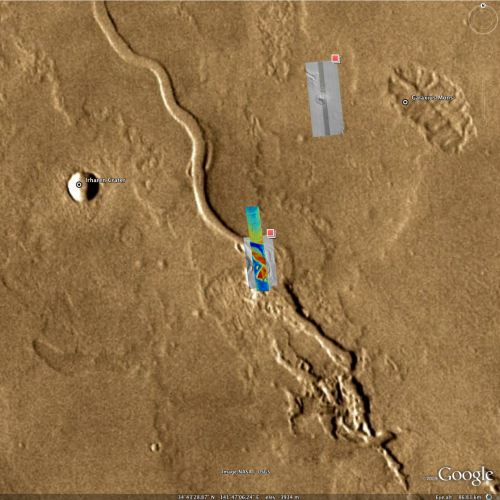
\includegraphics[width=6in]{images/p19-googlemars_500px.png}
\caption[Hrad shaded colorized DEM as a KML overlay] {
    \label{hrad-kml}
        The colorized hillshade DEM as a KML overlay.  }
\end{center}
\end{figure}

\subsection{Using DERT to Visualize Terrain Models}

The open source Desktop Exploration of Remote Terrain (DERT) software tool
can be used to explore large digital terrain models, like those created by
the Ames Stereo Pipeline.  For more information, visit \url{https://github.com/nasa/DERT}.


\chapter{Tips and Tricks}
\label{tips}

Here we summarize, in one place, some insights in how to get the most
from ASP, particularly the highest quality results in the smallest
amount of time.

\begin{itemize}
\item Ask for help or if you have questions. We're always glad to share
what we know, implement suggestions, and fix issues (section
\ref{get-help}).

\item Use the GUI (section \ref{stereo_gui}) to get comfortable with ASP
on a small region and to tune parameters (section \ref{stereo_gui}). A
solution specific to ISIS imagery is to crop your stereo pair (using the
ISIS \texttt{crop} command) to a small region of interest.

\item The highest quality results with ASP can be obtained with
  map-projected images (section \ref{mapproj-example}).

\item Run stereo on multiple machines (section \ref{parallel}).

\item Improve the quality of the inputs to get better outputs.
Bundle-adjustment can be used to find out the camera positions more
accurately (section \ref{baasp}). CCD artifact correction can be used
to remove artifacts from WorldView images (section
\ref{wvcorrect-example}). Jitter correction can be used for Digital
Globe imagery (section \ref{sec:jitter}).

\item Align the output point cloud to some known absolute reference with
\texttt{pc\_align} (section \ref{pc-align-example}).

\item Remove noise from the output point cloud. During stereo
triangulation, points that are further or closer than given distances
from planet center or left camera center can be removed as outliers
(section \ref{triangulation_options}). During DEM generation (section
\ref{point2dem}), points with large triangulation error can be removed
using \texttt{-\/-remove-outliers-params}. Spikes can be removed with
\texttt{-\/-median-filter-params}. Points close to the boundary, that
tend to be less accurate, can be eroded (\texttt{-\/-erode-length}).


\item During stereo filtering, islands can be removed with
\texttt{-\/-erode-max-size}.

\item Remove noise from the low-resolution disparity (D\_sub) that can
greatly slow down a run using  \texttt{-\/-rm-quantile-percentile} and
\texttt{-\/-rm-quantile-multiple}. Some care is needed with these to
not remove too much information.

\item Fill holes in output orthoimages for nicer display (also in DEMs),
during DEM and orthoimage generation with \texttt{point2dem} (section
\ref{point2dem}). Holes in an existing DEM can also be filled using
\texttt{dem\_mosaic} (section \ref{demmosaic}).

\item To get good results if the images lack large-scale features (such
as for ice plains) use a different way to get the low-resolution
disparity (section \ref{sparse-disp}).

\item If a run takes unreasonably long, decreasing the timeout parameter
may be in order (section \ref{longrun}).

\item Manually set the search range if the automated approach fails
(section \ref{sec:search_range}).

\item To increase speed, the image pair can be subsampled. For ISIS
imagery, the ISIS \texttt{reduce} command can be used, while for Digital
Globe data one can invoke the \texttt{dg\_mosaic} tool (section
\ref{dgmosaic}, though note that this tool may introduce aliasing). With
subsampling, you are trading resolution for speed, so this probably only
makes sense for debugging or ``previewing'' 3D terrain. That said,
subsampling will tend to increase the signal to noise ratio, so it may
also be helpful for obtaining 3D terrain out of noisy, low quality
images.

\item Photometric calibration (using the ISIS tools) can be used to improve the input images
and hence get higher quality stereo results.

\item If your images have missing or inaccurate camera pose information,
and they were acquired with frame (pinhole cameras), such data can be
solved for using structure-from-motion and bundle adjustment (chapter
\ref{ch:sfm}).

\item Shape-from-shading (chapter \ref{ch:sfs}) can be used to further
increase the level of detail of a DEM obtained from stereo, though this
is a computationally expensive process and its results are not easy to
validate.

\end{itemize}

We'll be happy to add here more suggestions from community's accumulated
wisdom on using ASP.
